% Architecture figure of the README. Build: pdflatex architecture.tex, then
% pdftoppm -png -r 200 -singlefile architecture.pdf architecture
\documentclass[border=6pt]{standalone}
\usepackage[T1]{fontenc}
\usepackage{lmodern}
\usepackage{tikz}
\usetikzlibrary{arrows.meta,positioning,fit,calc,backgrounds}

\definecolor{llmc}{RGB}{250,222,190}
\definecolor{retc}{RGB}{205,224,247}
\definecolor{kgc}{RGB}{208,236,208}
\definecolor{datc}{RGB}{238,238,238}

\tikzset{
  box/.style={draw, rounded corners=2pt, align=center, font=\small, minimum height=9mm, inner sep=3pt},
  llm/.style={box, fill=llmc},
  ret/.style={box, fill=retc},
  kg/.style={box, fill=kgc},
  dat/.style={box, fill=datc, rounded corners=0pt},
  arr/.style={-{Stealth[length=2mm]}, semithick},
  use/.style={-{Stealth[length=2mm]}, semithick, dashed, black!55},
  band/.style={draw=black!30, rounded corners=4pt, inner sep=5mm},
  bandlabel/.style={font=\bfseries\small, anchor=north west},
}

\begin{document}
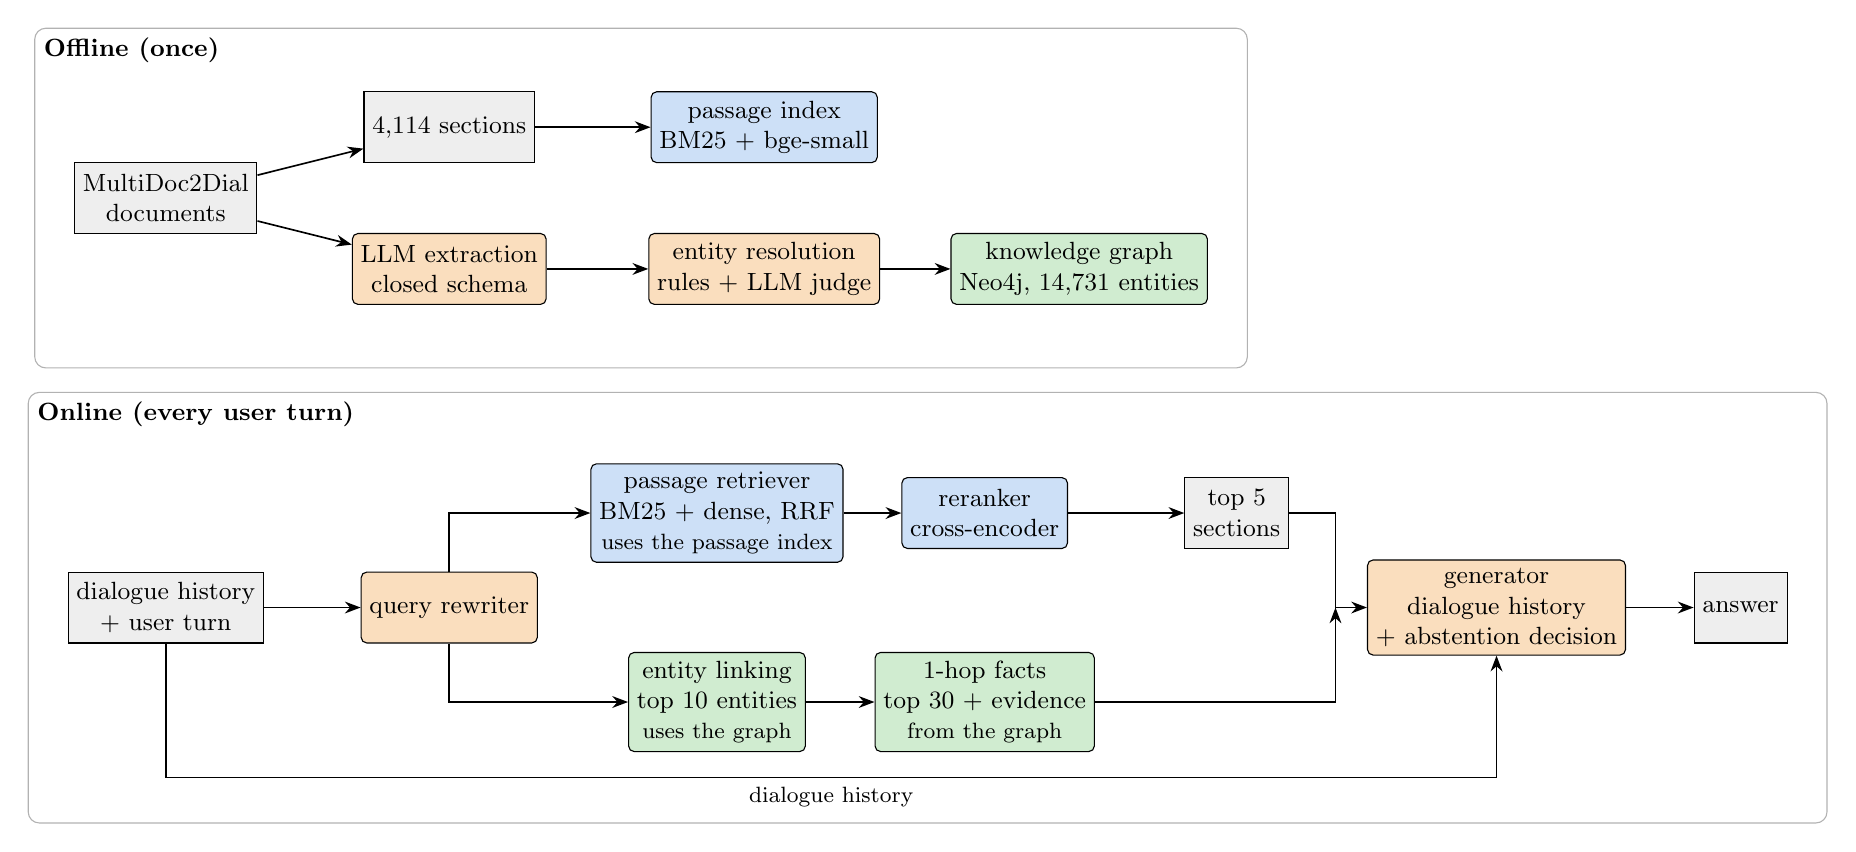
\begin{tikzpicture}
  % ---------------- offline ----------------
  \node[dat] (docs) at (0,0) {MultiDoc2Dial\\documents};
  \node[dat] (sec) at (3.6,0.9) {4,114 sections};
  \node[ret] (idx) at (7.6,0.9) {passage index\\BM25 + bge-small};
  \node[llm] (ext) at (3.6,-0.9) {LLM extraction\\closed schema};
  \node[llm] (er) at (7.6,-0.9) {entity resolution\\rules + LLM judge};
  \node[kg] (neo) at (11.6,-0.9) {knowledge graph\\Neo4j, 14,731 entities};
  \draw[arr] (docs) -- (sec); \draw[arr] (sec) -- (idx);
  \draw[arr] (docs) -- (ext); \draw[arr] (ext) -- (er); \draw[arr] (er) -- (neo);

  % ---------------- online ----------------
  \node[dat] (turn) at (0,-5.2) {dialogue history\\+ user turn};
  \node[llm] (rw) at (3.6,-5.2) {query rewriter};
  \node[ret] (pr) at (7.0,-4.0) {passage retriever\\BM25 + dense, RRF\\\footnotesize uses the passage index};
  \node[ret] (rr) at (10.4,-4.0) {reranker\\cross-encoder};
  \node[dat] (top) at (13.6,-4.0) {top 5\\sections};
  \node[kg] (el) at (7.0,-6.4) {entity linking\\top 10 entities\\\footnotesize uses the graph};
  \node[kg] (fa) at (10.4,-6.4) {1-hop facts\\top 30 + evidence\\\footnotesize from the graph};
  \node[llm] (gen) at (16.9,-5.2) {generator\\dialogue history\\+ abstention decision};
  \node[dat] (ans) at (20.0,-5.2) {answer};
  \draw[arr] (turn) -- (rw);
  \draw[arr] (rw) |- (pr); \draw[arr] (pr) -- (rr); \draw[arr] (rr) -- (top);
  \draw[arr] (rw) |- (el); \draw[arr] (el) -- (fa);
  \draw[arr] (top) -| ([xshift=-4mm]gen.west) -- (gen.west);
  \draw[arr] (fa) -| ([xshift=-4mm]gen.west);
  \draw[arr] (gen) -- (ans);
  \draw[arr] (turn.south) -- ++(0,-1.7) -| node[pos=0.25, below, font=\footnotesize] {dialogue history} (gen.south);


  \begin{scope}[on background layer]
    \node[band, fit=(docs)(sec)(idx)(ext)(er)(neo), inner ysep=8mm] (off) {};
    \node[band, fit=(turn)(rw)(pr)(rr)(top)(el)(fa)(gen)(ans), inner ysep=9mm] (on) {};
  \end{scope}
  \node[bandlabel] at (off.north west) {Offline (once)};
  \node[bandlabel] at (on.north west) {Online (every user turn)};
\end{tikzpicture}
\end{document}
